\documentclass[12pt]{article}
\usepackage[english]{babel}
\usepackage[utf8x]{inputenc}
\usepackage{amsmath}
\usepackage{graphicx}
\usepackage[colorinlistoftodos]{todonotes}
\pagenumbering{arabic} %numeracija stranica arapskim brojevima

\renewcommand{\refname}{Literatura} %da se zove literatura
% \renewcommand{\figurename}{Slika} % zelimo da nam label bude Slika, ne Figure
\usepackage{hyperref} %za linkovanje sadrzaja
\hypersetup{
    colorlinks=true,
    linktoc=all,
    linkcolor=blue,
} %za razlicite boje linkova

\usepackage{indentfirst}
\setlength{\parindent}{1cm}


\begin{document}

\begin{titlepage}

\newcommand{\HRule}{\rule{\linewidth}{0.5mm}} % Defines a new command for the horizontal lines, change thickness here

\center % Center everything on the page
 
%----------------------------------------------------------------------------------------
%	HEADING SECTIONS
%----------------------------------------------------------------------------------------

\textsc{\LARGE Matematički fakultet}\\[1.5cm] % Name of your university/college
\textsc{\Large Projekat iz predmeta Informacioni sistemi}\\[0.5cm] % Major heading such as course name
\textsc{\large Školska 2018/2019}\\[0.5cm] % Minor heading such as course title

%----------------------------------------------------------------------------------------
%	TITLE SECTION
%----------------------------------------------------------------------------------------

\HRule \\[0.4cm]
{ \huge \bfseries Poručivanje hrane }\\[0.4cm] % Title of your document
\HRule \\[1.5cm]
 
%----------------------------------------------------------------------------------------
%	AUTHOR SECTION
%----------------------------------------------------------------------------------------

\begin{minipage}{0.4\textwidth}
\begin{flushleft} \large
\emph{Author:}\\
John \textsc{Smith} % Your name
\end{flushleft}
\end{minipage}
~
\begin{minipage}{0.4\textwidth}
\begin{flushright} \large
\emph{Supervisor:} \\
Dr. James \textsc{Smith} % Supervisor's Name
\end{flushright}
\end{minipage}\\[2cm]

% If you don't want a supervisor, uncomment the two lines below and remove the section above
%\Large \emph{Author:}\\
%John \textsc{Smith}\\[3cm] % Your name

%----------------------------------------------------------------------------------------
%	DATE SECTION
%----------------------------------------------------------------------------------------

{\large \today}\\[2cm] % Date, change the \today to a set date if you want to be precise

%----------------------------------------------------------------------------------------
%	LOGO SECTION
%----------------------------------------------------------------------------------------


\includegraphics[width=40mm]{slike/logo.jpg}\\[1cm] % Include a department/university logo - this will require the graphicx package
 
%----------------------------------------------------------------------------------------

\vfill % Fill the rest of the page with whitespace

\end{titlepage}

\renewcommand{\contentsname}{Sadr\v zaj}
\thispagestyle{empty} %ovu stranu ne numerisemo
\tableofcontents %sadrzaj

\newpage
\renewcommand{\figurename}{Slika}
\section{Uvod}
Ovaj rad predstavlja informacioni sistem jednog restorana čiji se rad isključivo zasniva na isporuci porudžbina korisnicima. Izrađen je kao projekat u okviru predmeta "Informacioni sistemi" na master studijama Matematičkog fakulteta. Sistem obezbeđuje osnovne funkcionalnosti poput naručivanja hrane i pića, pripreme hrane, dostave, zatim interno upravljanje dobavljanjem i skladištenjem namirnica kao i koordinisanjem  svih zaposlenih u okviru restorana.
Za razliku od mnogih restorana koji pored poručivanja imaju i tu mogućnost da svoje korisnike i ugoste, to ovde nije slučaj, ali je moguće preuzimanje porudžbine u samom restoranu.

%ostaje dodati blize informacije iz prve ruke :D 

\section{Analiza sistema}
Cilj ovog sistema jeste da olakša funkcionisanje jednog on-line restorana. To se postiže međusobnom komunikacijom korisnika, koordinatora kao i oso\-ba zaduženih za pripremu i distribuciju hrane. Na taj način realizuju se zahtevi korisnika u najkraćem vremenskom roku sa što boljim kvalitetom usluga.
%\subsection{Dijagram konteksta}

Na narednoj slici (Slika \ref{fig:slika1}) nalazi se dijagram konteksta koji grafički prikazuje osnovne aktere u sistemu i veze medju njima.


% \begin{center}
% 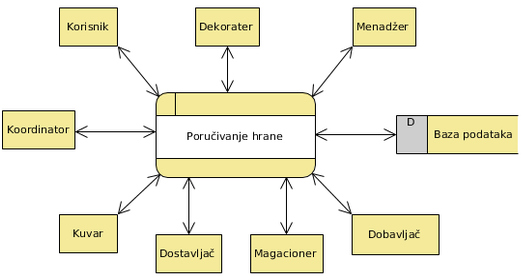
\includegraphics[width = 130mm]{slike/DC.jpg}
% \caption{Slika 1. Dijagram konteksta}
% \end{center}

\begin{figure}[ht]
    \leavevmode
    \begin{center}
    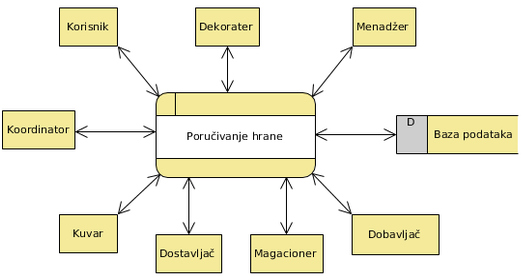
\includegraphics[height=0.3\textheight]{slike/DC.jpg}
    \end{center}
    \caption{Dijagram konteksta} % opis ce stajati ispod slike
    \label{fig:slika1}
\end{figure}


%Naime, korisniku je omogućeno da hranu naruči bilo putem telefona, bilo putem veb stranice.


%Ukoliko korisnik prvi put pristupa veb stranici radi naručivanja, neophodno je da se registruje sa ličnim podacima (ime, prezime, adresa, korisničko ime, lozinka...) dok svaki sledeći pristup stranici omogućen je običnom prijavom. Pored uobičajenih porudžbina, postoji i mogućnost aranžiranja i isporuke keteringa za različite tipove proslava.


%Sam restoran poseduje i sopstveni magacin za skladištenje svih potrebnih namirnica. Uz to, obezbeđeno je svo neophodno osoblje za koordinisanje ovakvog tipa restorana.


\subsection{Učesnici}
Glavna podela učesnika sistema je na:

\begin{itemize}
    \item Korisnik
    \begin{itemize}
        \item vrši porudžbine putem telefona ili veb stranice
        \item plaća dostavljaču utvrđeni iznos po prijemu paketa
        \item ocenjuje uslugu restorana
    \end{itemize}
    \item Koordinator
    \begin{itemize}
        \item prihvata ili odbacuje porudžbinu od korisnika
        \item u slučaju prihvatanja obaveštava kuvara o detaljima porudžbine
        \item po prijemu paketa od kuvara ili dekoratera, prosleđuje ga dostavljaču uz napomenu o adresi korisnika
    \end{itemize}
    \item Kuvar
    \begin{itemize}
        \item priprema hranu zahtevanu od strane koordinatora
        \item u slučaju da je porudžbina tipa keteringa, pripremljenu hranu prosleđuje dekorateru
        \item po potrebi, obaveštava magacionera o nedovoljnim zalihama namirnica u kuhinji
    \end{itemize}
    \item Dostavljač
    \begin{itemize}
        \item preuzima iz kuhinje paket koji treba isporučiti, zajedno sa adresom isporuke i cenom
        \item isporučuje paket na datu adresu u najkraćem vremenskom roku
        \item obaveštava korisnika o ceni, vrši naplatu isporučenih dobara
        \item po potrebi, obaveštava menadžera o nedovoljnim zalihama goriva/potrebnim popravkama na vozilu za isporuke
    \end{itemize}
        \item Menadžer
    \begin{itemize}
        \item vodi računa o prilivu i odlivu novca restorana
        \item koordinira zaposlenima i njihovim nalozima
    \end{itemize}
 
    \item Magacioner
    \begin{itemize}
        \item vodi računa o količini zaliha namirnica u magacinu
        \item vrši prenos zahtevanih namirnica, od strane kuvara, u kuhinju
        \item vrši skladištenje pristiglih namirnica u magacin
        \item koordinira isporukama sa dobavljačem
    \end{itemize}
    \item Dekorater
    \begin{itemize}
        \item sarađuje sa kuvarom u aranžiranju keteringa
        \item završenu porudžbinu prosleđuje koordinatoru
    \end{itemize}
    \item Dobavljač
    \begin{itemize}
        \item vrši prijem dobara od strane distributera
        \item vrši isporuku dobara u magacin
    \end{itemize}
\end{itemize}


Sledeci DTP dijagram (Slika \ref{fig:slika2}) nivoa jedan predstavlja osnovne celine koje smo uočili. 
% \begin{center}
% 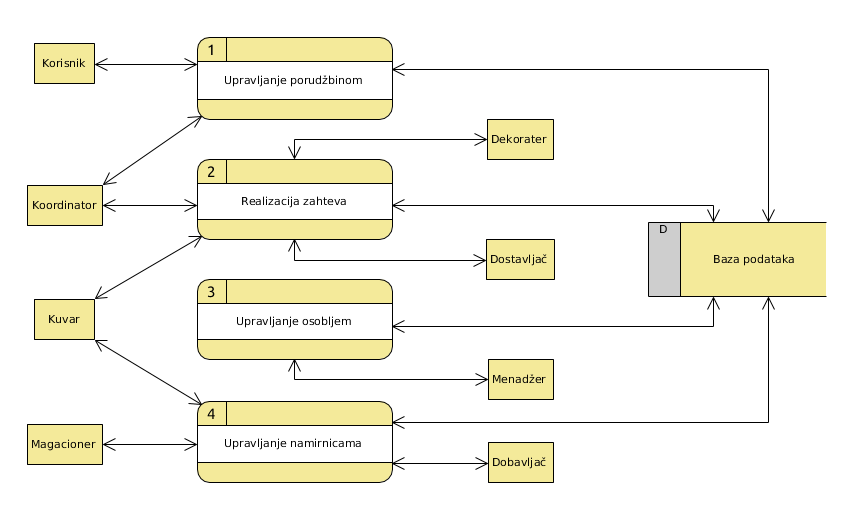
\includegraphics[width = 160mm]{slike/DTP.jpg}
% \caption{Slika 2. Dijagram toka podataka}
% \end{center}
\begin{figure}[ht]
    \leavevmode
    \begin{center}
    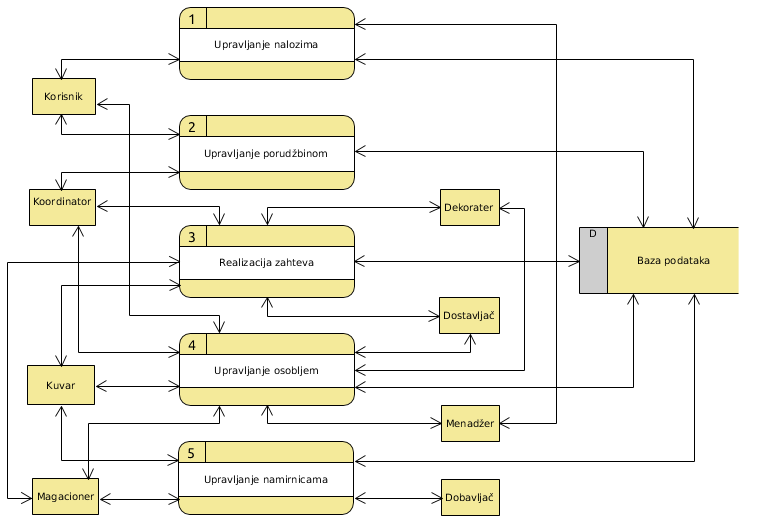
\includegraphics[height=0.4\textheight]{slike/DTP.png}
    \end{center}
    \caption{Dijagram toka podataka} % opis ce stajati ispod slike
    \label{fig:slika2}
\end{figure}

\newpage
\section{Slu\v cajevi upotrebe}
\subsection{Upravljanje nalozima}

\begin{figure}[ht]
    \leavevmode
    \begin{center}
    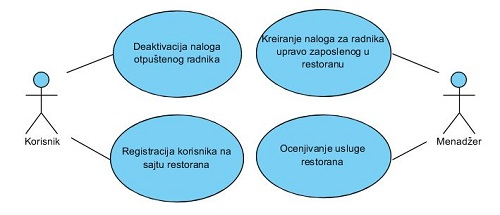
\includegraphics[width=1\textwidth]{slike/Upravljanje_nalozima.JPG}
    \end{center}
    \caption{Dijagram slučajeva upotrebe}
\end{figure}

\subsubsection{Registracija korisnika na sajtu restorana}
\begin{itemize}
    \item \textbf{Kratak opis}:
    Korisnik prvi put pristupa nalogu restorana i zato je neophodna registracija kako bi mogao poručiti hranu.
    \item \textbf{Učesnici}:
    Korisnik
    \item \textbf{Preduslovi}:
    Nema preduslova. 
    \item \textbf{Postuslovi}:
    Korisnik je registrovan. 
    \item \textbf{Glavni tok}:
    \begin{enumerate}
        \item Korisnik odlazi na nalog restorana i otvara formu za registraciju.
        \item Korisnik popunjava formu za registraciju.
        \item Sistem vrši validaciju registracije.
        \item Sistem beleži novog korisnika u bazi
        \item Sistem obaveštava korisnika o uspešnosti registracije.
    \end{enumerate}
\end{itemize}

\begin {itemize}
\item \textbf {Alternativni tokovi}: \\
 3.1. Korisnik nije uneo ispravne podatke za registraciju.\\
 Slučaj upotrebe se nastavlja na koraku 2 glavnog toka.
\end{itemize}
 \begin{itemize} 
    \item \textbf{Dodatne informacije}
    \begin{itemize}
        \item Neophodni podaci za registraciju korisnika su validna e-mail adresa, ime, prezime, adresa, korisničko ime i lozinka.
        \item Sistem validira novog korisnika tako što proverava da li već postoji nalog sa unetom e-mail adresom. Neophodno je i da korisničko ime bude jedinstveno.
    \end{itemize}
\end{itemize}
 
 
\subsubsection{Ocenjivanje usluge restorana}
\begin{itemize}
    \item \textbf{Kratak opis}:
    Korisniku je data mogućnost da napiše svoj utisak o usluzi restorana koji je vidljiv drugim korisnicima.
    \item \textbf{Učesnici}:
    Korisnik
    \item \textbf{Preduslovi}:
    Postojanje korisničkog naloga. 
    \item \textbf{Postuslovi}:
    Korisnik je napisao u komentaru svoj utisak
    o restoranu.
    \item \textbf{Glavni tok}:
   \begin{enumerate}
        \item Korisnik odlazi na nalog restorana i otvara stranicu Utisci.
        \item Korisnik popunjava formu za ostavljanje utiska.
        \item Sistem vrši validaciju utiska.
        \item Ažurira se stranica Utisci.
        \item Sistem obaveštava korisnika da je uspešno postavio komentar.
    \end{enumerate}
\end{itemize}
\begin{itemize}
\item \textbf {Alternativni tokovi}:\\ 
 3.1. Korisnik nije popunio sva obavezna polja.\\
 Slučaj upotrebe se nastavlja na koraku 2 glavnog toka.\\
 3.2. Korisnik je uneo e-mail adresu koja ne odgovara nijednom postojećem nalogu korisnika. \\
 Korisnik dobija odgovarajuću poruku i postavlja mu se pitanje da li želi da se registruje. \\
 Slučaj upotrebe se nastavlja na koraku 2 glavnog toka.
 
\quad 3.2.1. Korisnik potvrđuje da želi da se registruje.
Prelazi se na slučaj upotrebe ”3.1.1 Registracija korisnika na sajtu restorana".Nakon završetka tog slučaja upotrebe, slučaj upotrebe se vraća
na korak 2 glavnog toka. 

\quad 3.2.2. Korisnik ne želi da se registruje. Završava se slučaj upotrebe.
\end{itemize}

\begin{itemize} 
     \item \textbf{Dodatne informacije}
 \begin{itemize}
     \item Obavezna polja koja korisnik mora popuniti da bi ostavio utisak su validna e-mail adresa, ime i komentar.
    \item Sistem validira utisak tako što proverava da li postoji nalog korisnika kome odgovara uneta e-mail adresa.
 \end{itemize}
 \end{itemize}
 
 \subsubsection{Kreiranje naloga za radnika upravo zaposlenog u restoranu}
\begin{itemize}
    \item \textbf{Kratak opis}:
   Radniku koji je upravo zaposlen u restoranu potrebno je napraviti nalog kako bi imao pristup sistemu.
    \item \textbf{Učesnici}:
    Menadžer
    \item \textbf{Preduslovi}:
    Zaposleni je upravo dobio posao u restoranu.
    \item \textbf{Postuslovi}:
    Zaposleni ima svoj nalog. 
    \item \textbf{Glavni tok}:
   \begin{enumerate}
        \item Menadžer odlazi na veb stranicu i prijavljuje se unošenjem svog korisničkog imena i šifre.
        \item Menadžer otvara formu za unošenje novog naloga za zaposlene.
        \item Menadžer popunjava formu svim potrebnim podacima.
        \item Menadžer odredjuje prava pristupa nalozima zaposlenih.
        \item Menadžer potvrđuje unete podatke klikom na dugme 'Sačuvaj'.
        \item Sistem beleži novog zaposlenog u bazi.
        \item Sistem obaveštava zaposlenog o uspešnosti registracije slanjem e-mail poruke.
\end{enumerate}
\end{itemize}
\begin {itemize}
\item \textbf {Alternativni tokovi}:\\
 3.1. Menadžer nije uneo ispravne podatke za registraciju.\\
 Slučaj upotrebe se nastavlja na koraku 2 glavnog toka.
 \end{itemize}
 \begin{itemize} 
     \item \textbf{Dodatne informacije}
 \begin{itemize}
     \item Neophodni podaci za pravljenje naloga zaposlenom su validna e-mail adresa, ime, prezime, adresa, korisničko ime, lozinka, kao i odabir funkcije zaposlenog, čiji je nalog u nastanku.
    \item Sistem validira novog zaposlenog tako što proverava da li već postoji nalog sa unetom e-mail adresom. Neophodno je i da korisničko ime bude jedinstveno.
 \end{itemize}
 \end{itemize}

 \subsubsection{Deaktivacija naloga otpuštenog radnika}
 \begin{itemize}
    \item \textbf{Kratak opis}:
   Radniku koji je otpušten menadžer deaktivira nalog kako više ne bi imao pristup sistemu.
    \item \textbf{Učesnici}:
    Menadžer.
    \item \textbf{Preduslovi}:
    Radnik je dobio/dao otkaz u restoranu. Takođe, u sistemu postoji njegov nalog.
    \item \textbf{Postuslovi}:
    Radniku je deaktiviran nalog. 
    \item \textbf{Glavni tok}:
    \begin{enumerate}
        \item Menadžer odlazi na veb stranicu i prijavljuje se unošenjem svog korisničkog imena i šifre.
        \item Menadžer pronalazi nalog bivšeg zaposlenog.
        \item Menadžer deaktivira nalog klikom na dugme 'Deaktiviraj'.
        \item Menadžer potvrđuje unete promene klikom na dugme 'Sačuvaj'.
        \item Sistem beleži promene u bazi.
        \item Sistem obaveštava radnika o deaktivaciji naloga slanjem e-mail poruke.
    \end{enumerate}
\item \textbf{Dodatne informacije}
 \begin{itemize}
     \item Pri deaktivaciji naloga, nalog se ne briše, tako da u slučaju ponovnog zaposlenja, dovoljno je da menadžer aktivira postojeći nalog.
 \end{itemize}
 \end{itemize}
\newpage
\subsection{Upravljanje porudžbinom}
Na slici \ref{fig:slika3} je predstavljen dijagram stanja koji opisuje opšti tok upravljanja porudžbinom. U zavisnosti od toga da li među zalihama ima dovoljno namirnica, porudžbina se prihvata ili odbija.
\begin{figure}[ht]
    \leavevmode
    \begin{center}
    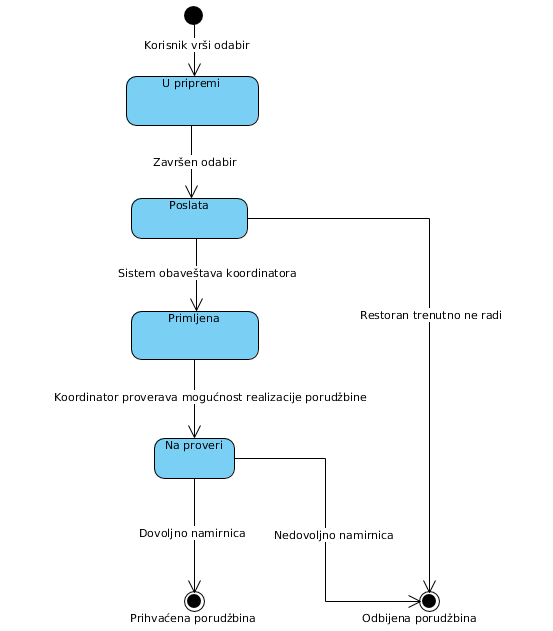
\includegraphics[height=0.6\textheight]{slike/Upravljanje_porudzbinom.png}
    \end{center}
    \caption{Dijagram stanja} % opis ce stajati ispod slike
    \label{fig:slika3}
\end{figure}


\subsubsection{Onlajn naručivanje}
\begin{itemize}
    \item \textbf{Kratak opis}: Korisnik naručuje željenu hranu putem veb stranice. Porudžbina biva prihvaćena ili odbijena od strane koordinatora.
    \item \textbf{Učesnici}: Korisnik, koordinator.
    \item \textbf{Preduslovi}: Postojanje korisničkog naloga.
    \item \textbf{Postuslovi}: Prihvaćena, odnosno odbijena porudžbina.
    \item \textbf{Glavni tok}:
    \begin{enumerate}
        \item Korisnik se prijavljuje na sajt restorana.
        \item Korisnik vrši odabir željenih proizvoda.
        \item Korisnik potvrđuje željenu porudžbinu klikom na dugme "Poruči".
        \item Sistem odbija porudžbinu u slučaju da restoran trenutno ne radi i obaveštava korisnika o tome.
        \item Sistem obaveštava koordinatora o prispeću zahteva.
        \item Koordinator proverava da li je moguće realizovati porudžbinu.
        \item Koordinator utvrđuje da svih namirnica potrebnih za datu porudžbinu ima u dovoljnim količinama.
        \item Koordinator beleži na cedulju detalje porudžbine.
        \item Koordinator prihvata porudžbinu klikom na dugme "Prihvati".
        \item Korisnik biva obavešten, od strane sistema, da je porudžbina prihvaćena ili ne.
     \end{enumerate}
     \item \textbf{Alternativni tokovi}:
     
     7.1. Koordinator utvrđuje da ne postoji dovoljna količina namirnica za pripremu porudžbine. Slučaj upotrebe se nastavlja na koraku 9.1.\\
     9.1. Koordinator odbija porudžbinu klikom na dugme "Odbij". Slučaj upotrebe se nastavlja  nastvlja na koraku 10 glavnog toka.\\
     7.2. Koordinator proverava da li je vrednost parudžbine veća od definisane vrednosti za poklon uz porudžbinu. Slučaj upotrebe se nastavlja na koraku 8.1.\\
     8.1. Koordinator beleži na cedulju dodatak porudžbini koji korisnik dobija kao poklon. Slučaj upotrebe se nastavlja na koraku 9 glavnog toka.\\
    
\end{itemize}

\subsubsection{Naručivanje telefonom}

\begin{figure}[ht]
    \leavevmode
    \begin{center}
    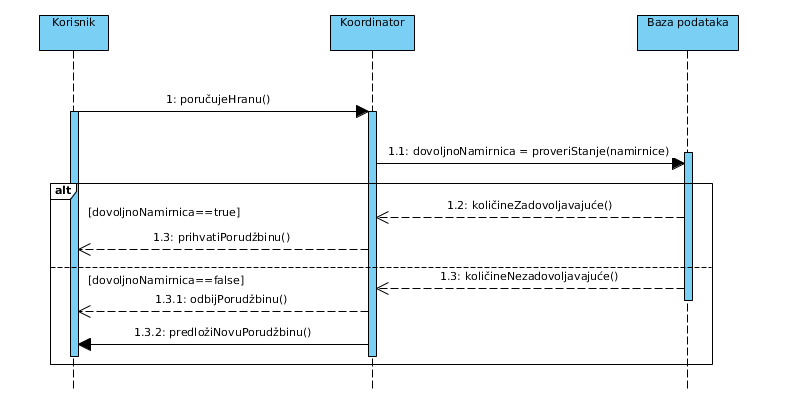
\includegraphics[width=125mm]{slike/DijagramSekvenci.png}\\
    \end{center}
    \caption{Dijagram slučajeva upotrebe}
\end{figure}


\begin{itemize}
    \item \textbf{Kratak opis}: Korisnik naručuje željenu hranu pozivom na telefon restorana. Porudžbina biva prihvaćena ili odbijena od strane koordinatora.
    \item \textbf{Učesnici}: Korisnik, koordinator.
    \item \textbf{Preduslovi}: Postojanje registrovanog telefonskog aparata u restoranu.
    \item \textbf{Postuslovi}: Prihvaćena, odnosno odbijena porudžbina.
     \item \textbf{Glavni tok}:
    \begin{enumerate}
        \item Korisnik vrši poziv restorana.
        \item Korisnik vrši odabir željenih proizvoda.
        \item Koordinator proverava da li je moguće realizovati porudžbinu, odnosno
        da li ima dovoljno namirnica potrebnih za datu porudžbinu.
        \item Koordinator prihvata porudžbinu i saopštava korisniku.
        \item Korisnik biva obavešten, od strane koordinatora, da je porudžbina prihvaćena.
    \end{enumerate}
    \item \textbf{Alternativni tokovi}:\\
     1.1. Korisnik biva obavešten, od strane telefonske sekretarice, da restoran trenutno ne radi. Slučaj upotrebe se ovde završava.\\
     4.1. Koordinator utvrđuje da ne postoji dovoljna količina namirnica za pripremu porudžbine. Slučaj upotrebe se nastavlja na koraku 5.1.\\
     5.1. Koordinator odbija porudžbinu i saopštava korisniku. Koordinator korisniku nudi mogućnost da poruči nešto drugo.  
     
      \quad 5.1.1. Korisnik želi da poruči nešto drugo. Slučaj upotrebe se nastavlja na koraku 2 glavnog toka. 
      
      \quad 5.1.2. Korisnik ne želi da poruči nešto drugo. Slučaj upotrebe se završava. \\
    
    \end{itemize}
    
Na narednoj slici nalazi se dijagram slučaja upotrebe kojim se prikazuje interakcija izmedju korisnika i koordinatora prilikom naručivanja hrane, bilo putem telefona ili onlajn.

\begin{figure}[ht]
    \leavevmode
    \begin{center}
    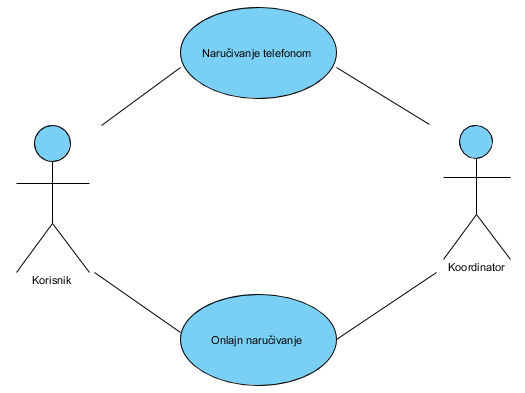
\includegraphics[height=0.5\textheight]{slike/Upravljanje_porudzbinomUC.png}
    \end{center}
    \caption{Dijagram slučaja upotrebe}
\end{figure}


\newpage
\subsection{Realizacija zahteva}
\begin{figure}[ht]
    \leavevmode
    \begin{center}
    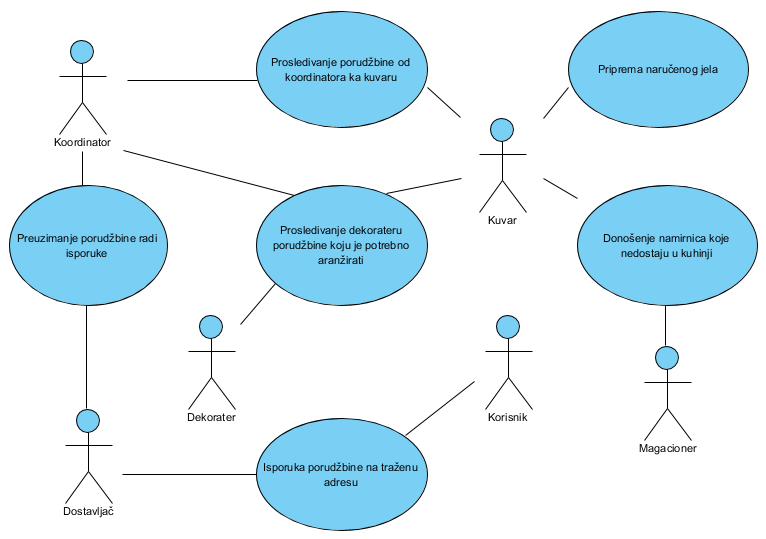
\includegraphics[height=0.55\textheight]{slike/Realizacija_zahteva.png}
    \end{center}
    \caption{Dijagram slu\v cajeva upotrebe} % opis ce stajati ispod slike
    \label{fig:slika4}
\end{figure}
 \begin{figure}[ht]
    \leavevmode
    \begin{center}
    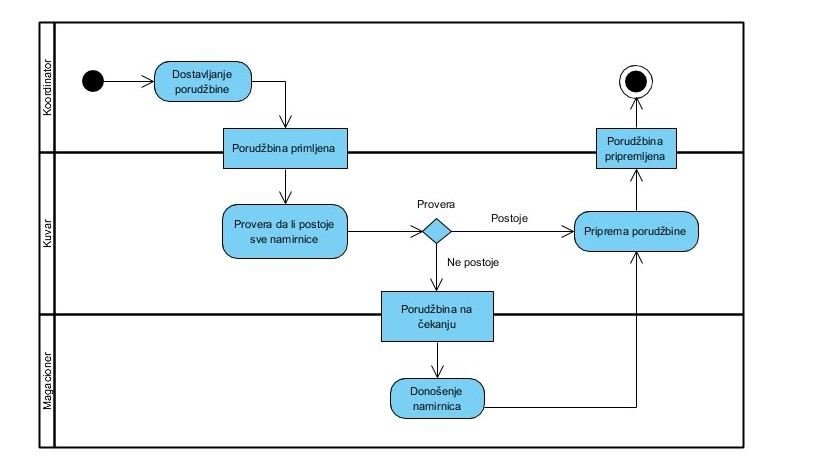
\includegraphics[height=0.35\textheight]{slike/Realizacija_zahteva_dijagram_aktivnosti.jpg}
    \end{center}
    \caption{Dijagram aktivnosti} % opis ce stajati ispod slike
    \label{fig:slika6}
\end{figure}
\subsubsection{Prosleđivanje porudžbine od koordinatora ka kuvaru}
\begin{itemize}
    \item \textbf{Kratak opis}:
    Koordinator prosledjuje zahtev za pripremu naručene hrane kuvaru.
    \item \textbf{Učesnici}:
    Koordinator, kuvar.
    \item \textbf{Preduslovi}:
    Postoje sve neophodne namirnice za pripremu poručenog jela.
    \item \textbf{Postuslovi}:
    Kuvar je primio zahtev za porudžbinom.
    \item \textbf{Glavni tok}:
   \begin{enumerate}
        \item Koordinator ostavlja cedulju sa naručenim jelom na glavni pult kuhinje. Cedulja sadrži i informaciju o adresi isporuke i ceni kao i podatak da li je porudžbina namenjena za ketering.
        \item Kooordinator usmeno obaveštava kuvara da postoji nova porudžbina.
        \item Kuvar preuzima cedulju sa informacijama o porudžbini.
\end{enumerate}
\end{itemize}

\subsubsection{Priprema naručenog jela}
\begin{itemize}
    \item \textbf{Kratak opis}:
    Kuvar priprema jelo koje je prethodno naručeno.
    \item \textbf{Učesnici}:
    Kuvar.
    \item \textbf{Preduslovi}:
    Nema preduslova.
    \item \textbf{Postuslovi}:
    Kuvar je pripremio jelo.
    \item \textbf{Glavni tok}:
   \begin{enumerate}
        \item Kuvar utvrđuje da li u kuhinji postoje sve namirnice koje
        su mu neophodne za pripremu porudžbine.
        \item Kuvar prikuplja namirnice koje će koristiti za pripremu hrane.
        \item Kuvar priprema naručenu hranu.
        \item Kuvar obaveštava koordinatora da je
        jelo pripremljeno.
\end{enumerate}
 \item \textbf{Alternativni tokovi}:\\
     1.1. Kuvar je utvrdio da u kuhinji ne postoje
     sve namirnice koje su neophodne.
     \\ Prelazi se na slučaj
    upotrebe "3.3.3 Donošenje namirnica koje nedostaju u kuhinji". Nakon završetka tog slučaja upotrebe, slučaj upotrebe se
    vraća na korak 2 glavnog toka. 
\end{itemize}

\subsubsection{Donošenje namirnica koje nedostaju u kuhinji}
\begin{itemize}
    \item \textbf{Kratak opis}:
    Magacioner donosi u kuhinju namirnice koje su kuvaru potrebne za pripremu hrane.
    \item \textbf{Učesnici}:
    Magacioner, kuvar.
    \item \textbf{Preduslovi}:
    Nema preduslova.
    \item \textbf{Postuslovi}:
    Kuvar ima u kuhinji sve namirnice koje su mu potrebne za pripremu jela koje je poručeno.
    \item \textbf{Glavni tok}:
   \begin{enumerate}
        \item Kuvar poziva magacionera i zahteva iz magacina namirnice koje mu nedostaju.
        \item Magacioner prikuplja tražene namirnice.
        \item Magacioner donosi u kuhinju namirnice.
\end{enumerate}
\end{itemize}

\subsubsection{Prosleđivanje dekorateru porudžbine koju je potrebno aranžirati}
\begin{itemize}
    \item \textbf{Kratak opis}:
    Dekorater aranžira hranu koja je
    namenjena za ketering.
    \item \textbf{Učesnici}: 
    Dekorater, koordinator, kuvar.
    \item \textbf{Preduslovi}:
    Porudžbina je pripremljena i spremna
    za aranžiranje.
    \item \textbf{Postuslovi}:
    Dekorater je aranžirao ketering.
    \item \textbf{Glavni tok}:
   \begin{enumerate}
        \item Kuvar obaveštava koordinatora da
        je porudžbina pripremljena i može da 
        se aranžira.
        \item Koordinator obaveštava
        dekoratera da postoji porudžbina koju je potrebno aranžirati.
        \item Dekorater preuzima porudžbinu i aranžira je.
        \item Dekorater javlja koordinatoru da 
        je porudžbina dekorisana i spremna za isporuku.
\end{enumerate}
\end{itemize}


\subsubsection{Preuzimanje porudžbine radi isporuke}
\begin{itemize}
    \item \textbf{Kratak opis}:
    Dostavljač preuzima iz kuhinje paket koji je potrebno isporučiti na adresu korisnika.
    \item \textbf{Učesnici}: 
    Koordinator, dostavljač.
    \item \textbf{Preduslovi}:
    Porudžbina je već pripremljena i aranžirana ukoliko je postojao zahtev za aranžmanom.
    \item \textbf{Postuslovi}:
    Dostavljač je primio paket koji treba isporučiti.
    \item \textbf{Glavni tok}:
   \begin{enumerate}
        \item Kooordinator obaveštava
        dostavljača da postoji porudžbina koju 
        treba da dostavi.
        \item Dostavljač preuzima iz kuhinje paket koji treba isporučiti zajedno sa ceduljom na kojoj se nalazi informacija o adresi isporuke i ceni.
\end{enumerate}
\end{itemize}

 \subsubsection{Isporuka porudžbine na traženu adresu}
 \begin{itemize}
    \item \textbf{Kratak opis}: Dostavljač vrši dostavu paketa korisniku i naplaćuje uslugu.
    \item \textbf{Učesnici}:
    Dostavljač, korisnik.
    \item \textbf{Preduslovi}:
    Postoji slobodan dostavljač za vršenje isporuke.
    \item \textbf{Postuslovi}:
    Korisnik je primio paket.
    \item \textbf{Glavni tok}:
    \begin{enumerate}
        \item Dostavljač dolazi na traženu adresu.
        \item Dostavljač obaveštava korisnika putem telefona da je porudžbina stigla.
        \item Korisnik se sastaje sa dostavljačem.
        \item Korisnik plaća uslugu gotovinom ili karticom.
        \item Dostavljač predaje paket korisniku.
 \end{enumerate}
    \item \textbf{Alternativni tokovi}:\\
        2.1. Dostavljač ne može dobiti korisnika. Čekaće maksimum deset minuta; ukoliko do tada ne stupi u kontakt sa korisnikom, paket se vraća u restoran. 
        
        \quad 2.1.1. Dostavljač je kontaktirao korisnika. Slučaj upotrebe se nastavlja na koraku 3 glavnog toka.
        
        \quad 2.1.2. Dostavljač ni posle deset minuta nije stupio u kontakt sa korisnikom. Slučaj upotrebe se završava.
        
    \item \textbf{Dodatne informacije}:
     \begin{itemize}
     \item U slučaju da korisnik plaća gotovinom, a dostavljač nema sitan novac za vraćanje kusura, u obavezi je da u najkraćem roku u blizini nađe sitan novac.
 \end{itemize}
 \end{itemize}
 \newpage
 \subsection{Upravljanje osobljem}
 Upravljanje osobljem predstavlja podno\v senje i obradu zahteva za odmorom ili nepla\'cenim odmorom, kao i njihovo evidentiranje u sistem. U ovim slu\v cajevima upotrebe u\v cesnici su menad\v zer i bilo koji zaposleni.
 
 \begin{itemize}
     \item Zaposleni zahteva odredjeni broj dana za odmor ili nepla\' ceni odmor na osnovu toga da li ima na raspolaganju dane za odmor ili ne.
     \item Zadu\v zenje menad\v zera je da prispele zahteve obradi, po\v salje odgovor, kao i da sve to evidentira u sistemu.
 \end{itemize}
 \begin{figure}[!ht]
    \leavevmode
    \begin{center}
    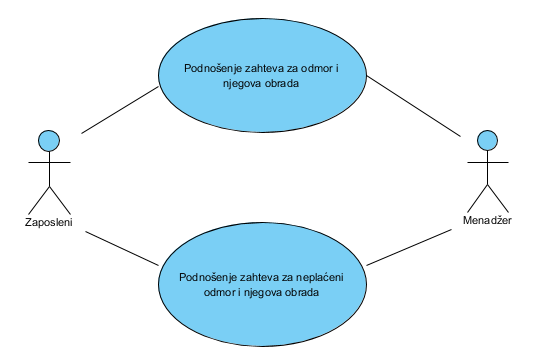
\includegraphics[height=0.45\textheight]{slike/Upravljanje_osobljem.png}
    \end{center}
    \caption{Dijagram slu\v cajeva upotrebe} % opis ce stajati ispod slike
    \label{fig:slika7}
\end{figure}
  \subsubsection{Podno\v senje zahteva za odmor i njegova obrada }
 \begin{itemize}
    \item \textbf{Kratak opis}:
   Zaposleni podnosi zahtev za odmor. Menad\v zer obra\dj uje njegov zahtev.
    \item \textbf{Učesnici}:
    Zaposleni, menad\v zer
    \item \textbf{Preduslovi}: Zaposleni ima na raspolaganju dane za odmor.
    \item \textbf{Postuslovi}:
    Zaposlen je obave\v sten da li je njegov zahtev prihva\'cen ili ne.
    \item \textbf{Glavni tok}:
    \begin{enumerate}
        \item Zaposleni se prijavljuje na sistem
        \item Zaposleni vr\v si odabir odre\dj enih datuma za odmor
        \item Zahtev za odmor se evidentira u sistemu 
        \item Sistem obave\v stava menad\v zera da je stigao zahtev za odmor slanjem e-mail poruke
        % \item Menad\v zer je obave\v sten da je primio zahtev za odmor ili nepla\'ceni odmor (e-mail).
        \item Menad\v zer se prijavljuje na sistem
        \item Menad\v zer proverava da li je moguće organizovati funkcionisanje objekta za odre\dj ene datume bez dotičnog zaposlenog
        \item Na osnovu procene stanja menad\v zer donosi odluku i to se evidentira u sistemu.
        \item Sistem prera\v cunava i a\v zurira preostale dane za odmor zaposlenog
        \item Sistem obave\v stava zaposlenog da je stigao odgovor na zahtev za odmor slanjem e-mail poruke.
        \item Zaposleni dobija informaciju da li je njegov zahtev odobren ili ne
    \end{enumerate}
\item \textbf{Alternativni tokovi}\\
        3.1. Uneti datumi nisu validni, sistem prosleđuje poruku za ponovno unošenje datuma, nakon čega se slučaj upotrebe nastavlja na koraku 3 glavnog toka.

 \end{itemize}
 
 \subsubsection{Podno\v senje zahteva za nepla\'ceni odmor i njegova obrada }
 \begin{itemize}
    \item \textbf{Kratak opis}:
  Zaposleni podnosi zahtev za nepla\'ceni odmor. Menad\v zer obra\dj uje njegov zahtev.
    \item \textbf{Učesnici}:
    Zaposleni, menad\v zer
    \item \textbf{Preduslovi}: Nema
    \item \textbf{Postuslovi}:
    Zaposlen je obave\v sten da li je njegov zahtev prihva\'cen ili ne.
    \item \textbf{Glavni tok}:
    \begin{enumerate}
        \item Zaposleni se prijavljuje na sistem
        \item Zaposleni vr\v si odabir odre\dj enih datuma za nepla\'ceni odmor.
        \item Zahtev za nepla\'ceni odmor se evidentira u sistemu.
        \item Sistem obave\v stava menad\v zera da je stigao zahtev za nepla\'ceni odmor slanjem e-mail poruke.
        \item Menad\v zer se prijavljuje na sistem.
        \item Menad\v zer proverava da li je moguće organizovati funkcionisanje objekta za odre\dj ene datume bez dotičnog zaposlenog.
        \item Sistem prera\v cunava i a\v zurira platu za zaposlenog.
        \item Sistem obave\v stava zaposlenog da je stigao odgovor na zahtev za nepla\'ceni odmor slanjem e-mail poruke.
        \item Zaposleni dobija informaciju da li je njegov zahtev odobren ili ne.
    \end{enumerate}
\item \textbf{Alternativni tokovi}\\
        2.1. Uneti datumi nisu validni, sistem prosleđuje poruku za ponovno unošenje datuma, nakon čega se slučaj upotrebe nastavlja na koraku 2 glavnog toka.

\end{itemize}
  
 
 \subsection{Upravljanje namirnicama}
 Upravljanje namirnicama podrazumeva vođenje računa o zalihama hrane i pića u restoranu. Ovo je neophodno da bi bilo koji restoran mogao da funkcioniše. Odnosi se na poručivanje hrane, prijem robe i evidentiranje prispele robe u sistemu. U ovom procesu učestvuju magacioner i dobavljač.
 Na Slici \ref{fig:slika5} predstavljen je dijagram slučajeva upotrebe za upravljanje namirnicama.
 
 \begin{itemize}
     \item Magacioner na osnovu stanja namirnica u magacinu sastavlja spisak za nabavku i obaveštava dobavljača o porudžbini. Kada roba pristigne, smešta je u magacin i evidentira prispeće robe u sistemu.
     \item Dobavljač isporučuje namirnice restoranu.
 \end{itemize}

% 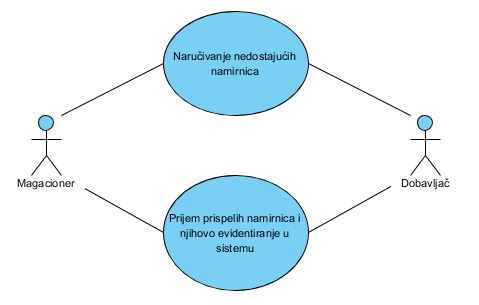
\includegraphics[width=136mm]{slike/Upravljanje_namirnicama.JPG}\\
% \begin{center}
% \caption{Slika 7. Dijagram slučajeva upotrebe}
% \end{center}
\begin{figure}[ht]
    \leavevmode
    \begin{center}
    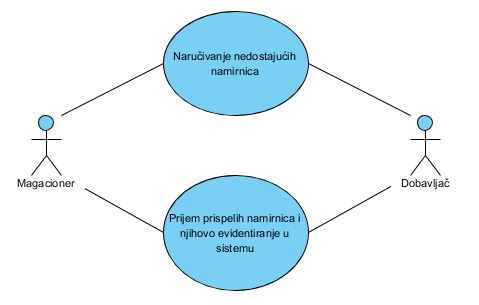
\includegraphics[height=0.5\textheight]{slike/Upravljanje_namirnicama.JPG}
    \end{center}
    \caption{Dijagram slu\v cajeva upotrebe} % opis ce stajati ispod slike
    \label{fig:slika8}
\end{figure}
 
 
 
 
 
 
 \subsubsection{Naručivanje nedostajućih namirnica}
 \begin{itemize}
    \item \textbf{Kratak opis}:
   Magacioner od dobavljača naručuje namirnice koje nedostaju u magacinu.
    \item \textbf{Učesnici}:
    Magacioner, dobavljač
    \item \textbf{Preduslovi}:
    U magacinu nedostaje izvesna količina određenih namirnica.
    \item \textbf{Postuslovi}:
    Dobavljaču je obavešten o količini i tipu namirnica koje treba da dobavi. 
    \item \textbf{Glavni tok}:
    \begin{enumerate}
        \item Magacioner pregledom inventara u sistemu utvrđuje da izvesna količina namirnica nedostaje.
        \item Magacioner pravi spisak koji sadrži sve namirnice koje će poručiti.
        \item Magacioner poziva dobavljača i poručuje namirnice sa spiska.
        \item Dobavljač saopštava magacioneru koje namirnice može u kom vremenskom roku da mu isporuči.
        \item Magacioner potvrđuje svoju porudžbinu.
    \end{enumerate}
\item \textbf{Alternativni tokovi}\\
        5.1. Magacioner otkazuje svoju porudžbinu. Slučaj upotrebe se nastavlja\\ na koraku 3 glavnog toka.
 
 \item \textbf{Dodatne informacije}
 \begin{itemize}
     \item 
    Magacioner otkazuje porudžbinu u slučaju da mu vremenski rok\\ koji mu dobavljač predlaže ne odgovara. Zatim poziva drugog dobavljača kako bi poručio namirnice.

 \end{itemize}
 \end{itemize}
 
  \subsubsection{Prijem prispelih namirnica i njihovo evidentiranje u sistemu}
 \begin{itemize}
    \item \textbf{Kratak opis}:
   Dobavljač isporučuje poručenu robu magacioneru. Magacioner smešta namirnice u magacin i evidentira nabavku u sistemu.
    \item \textbf{Učesnici}:
    Magacioner, dobavljač
    \item \textbf{Preduslovi}:
    Magacioner je poručio namirnice od dobavljača.
    \item \textbf{Postuslovi}:
    Magacin je dopunjen nedostajućim namirnicama i stanje magacina je ažurirano u sistemu. 
    \item \textbf{Glavni tok}:
    \begin{enumerate}
        \item Dobavljač pristiže na adresu restorana.
        \item Dobavljač obaveštava magacionera da je stigao.
        \item Dostavljač i magacioner se sastaju.
        \item Magacioner plaća dostavljaču.
        \item Dostavljač predaje robu magacioneru.
        \item Magacioner smešta robu u magacin.
        \item Magacioner u sistemu evidentira pristiglu nabavku.
        \item Sistem ažurira stanje namirnica u magacinu.  
        
    \end{enumerate}

\end{itemize}
 
 


\section{Opis baze podataka}
Informacioni sistem  restorana osmišljen je tako da umnogome olakša poslovanje samog restorana, rad zaposlenih u njemu kao i komunikaciju izmedju zaposlenih. Jedan od najbitnijih aspekata ovog informacionog si\-stema je upravo baza podataka. Pravilno dizajnirana baza podataka pruža njegovim korisnicima pristup ažuriranim, tačnim informacijama. \\
\indent Baza podataka je projektovana tako da pokriva sve slučajeve upotrebe informacionog sistema. \\
\indent U bazi postoji apstraktni tip eniteta \textbf{Osoba} iz kog su izvedeni tipovi entiteta  \textbf{Zaposleni} i \textbf{Korisnik} koji opisuju redom skup zaposlenih u restoranu i skup registrovanih korisnika restorana, tim redom. \\

Tabela \textbf{Osoba} sadrži zajedničke informacije za zaposlene i korisnike. Polje "id\_osobe" se odnosi na jedinstveno korisničko ime, a "aktivan" označava da li je zaposleni korisnik trenutno aktivan (bit 1) na nalogu restorana ili ne (bit 0). \\

\indent Registracijom korisnika na sajtu restorana dodaje se red u tabeli \textbf{Oso\-ba}. Apstraktni entitet \textbf{Osoba} se specijalizuje entitetom \textbf{Korisnik} i tabela \textbf{Korisnik} se popunjava odgovarajućim redom. \\

Slično, kreiranjem naloga za novog radnika se apstraktni entitet \textbf{Osoba} specijalizuje entitetom \textbf{Zaposleni} i tabela \textbf{Zaposleni} se popunjava odgovarajućim redom. Ova tabela povezana je sa tabelom \textbf{Uloga} ključem koji ukazuje na odgovarajuću poziciju u sistemu zaposlenih.\\

Deaktivacija naloga otpuštenog radnika vrši se samo promenom bita sa 1 na 0 u polju "aktivan" tabele \textbf{Osoba}.\\

Svaki korisnik ima pravo da ostavi utisak o kvalitetu usluge restorana. Ocenjvanje usluge restorana vrši se na osnovu polja "Jeloid\_jela" u tabeli \textbf{Ocena}. To je ujedno i strani kluč koji se odnosi na tabelu \textbf{Jelo}. Polje "vrednost" ukazuje na ocenu, a komentar nije obavezan. Tabela \textbf{Ocena} je povezana stranim ključem "KorisnikOsobaid\_osobe" i sa tabelom \textbf{Korisnik}. \\

Prilikom naručivanja (online ili telefonom) dodaje se novi red u tabeli \textbf{Porudžbina} pod uslovom da je porudžbina prihvaćena. Takodje, u tabeli se bele\v zi i da li je u pitanju ketering ili ne (kolona "ketering"). Tabela je povezana sa tabelom \textbf{Korisnik} identifikatorom osobe kao i sa tabelom \textbf{Spisak} identifikatorom porudžbine. Da bi se proverila mogućnost realizacije porudžbine, dodaje se najpre novi red u tabeli \textbf{Spisak} sa traženim zahtevima. Koordinator proverava preko identifikatora jela i namirnica da li ima dovoljno zaliha trenutno u magacinu. Identifikatori jela i namirnica su povezani tabelom \textbf{Priprema}. Napomena: identifikator jela se odnosi kako na hranu, tako i na piće.
\\

U toku realizacije porud\v zbine, sve neophodne namirnice za pripremu naru\v cenog jela, koje nedostaju u kuhinji, magacioner donosi kuvaru. Dono\v senje svih tih namirnica prouzrokuje a\v zuriranje kolone "kvantitet" u tabeli \textbf{Namirnice}. Za svaku namirnicu pojedina\v cno se imanjuje njen kvantitet u magacinu.\\

\indent Kad kuvar zavr\v si pripremu bilo kog jela sa dobijenog spiska, on o tome obavesti koordinatora. Pritom se a\v zurira kolona "spremljeno" u tabeli \textbf{Spisak} za to jelo (postavlja se na 1). Kada su sva jela sa spiska porud\v zbine pripremljena, ukoliko je data porud\v zbina u vidu keteringa, kuvar obave\v stava koordinatora, a ovaj dekoratera da je sve spremno za dekoraciju. Nakon zavr\v sene dekoracije, porud\v zbina je spremna za dostavu i o tome je, naravno, obave\v sten koordinator. To se u bazi evidentira tako \v sto se kolona "pripre\-mljena" u tabeli \textbf{Porud\v zbina} postavi na 1 za datu porud\v zbinu.\\

\indent Pripremljenu porud\v zbinu koju je zahtevao korisnik isporu\v cuje dostavlja\v c. Tom prilikom se kreira novi red u tabeli \textbf{Dostava}. Ova tabela sadr\v zi podatke o porud\v zbini, preko stranog kljuca "Porudzbinaid\_porudzbine" na tabelu \textbf{Porud\v zbina}, zatim o zaposlenom (dostavlja\v cu) preko stranog klju\v ca "ZaposleniOsobaid\_osobe" na tabelu  \textbf{Zaposleni}, kao i informacije o vremenu polaska, vremenu dostave i o tome da li je dostava uspe\v sno realizovana ili nije. Primarni klju\v c je par: id\_porudzbine, id\_osobe.\\
\indent Dostava je uspe\v sno realizovana ukoliko je dostavljena datom korisniku (kolona "uspesna" u tabeli \textbf{Dostava} se postavlja na 1).\\

Zaposleni ima pravo da podnese zahtev za odmorom ili nepla\'cenim odustvom. Svaki ovaj zahtev implicira unošenje novog reda u tabelu \textbf{Zahtev za odsustvom}. Ova tabela jedinstveno je odredjena identifikatorom odsustva i korisničkim imenog zaposlenog i ujedno je stranim klju\v cem povezana sa tabelom Zaposleni. Zaposleni podnosi zahtev za nepla\'cenim odmorom u slučaju da nema više slobodnih dana, i u tom slučaju polje "plaćeno" u odgovarajućem redu tabele biće 0. U suprotnom, tj. ukoliko zaposleni može podneti zahtev za odmorom, polje  "plaćeno" imaće vrednost 1. \\
\indent U zavisnosti od toga da li je zahtev radnika za odsustvom ili odmorom prihvaćen ili odbijen, polje "odobreno" imaće vrednost 1 ili 0. \\

Tabela \textbf{Namirnice} sadrži osnovne informacije o namirnicama u magacinu. Zaposleni magacioner vodi računa o zalihama namirnica i na osnovu podataka u ovoj tabeli zna kada i kojim namirnicama treba snabdeti magacin. \\ 
\indent Ova tabela kao primarni ključ ima kolonu "id\_namirnice". Kolona "količina" čuva podatak o količini  jednog pakovanja dotične namirnice, a kolona "merna\_jedinica"
u skladu s tim, kojom mernom jedinicom se mere pakovanja. Kolona "kvantitet" prikazuje brojno stanje pakovanja te namirnice.
Kada polje "kvantitet" ima vrednost manju od polja "minimum" u tabeli \textbf{Namirnice} u redu čiji je identifikator id\_namirnice baš te namirnice, magacioner zna da je ta namirnica na isteku svojih zaliha i da ju je potrebno naručiti. \\
\indent Kako se menja stanje namirnice u magacinu tako se ažurira i polje "kvantitet" i postavlja na vrednost trenutnog stanja te namirnice u maga\-cinu.
\href{https://raw.githubusercontent.com/JelenaCosic1994/Porucivanje_hrane/master/slike/Baza.jpg}{Ovde} se nalazi slika veće rezolucije.

\begin{figure}[!h]
    \leavevmode
    \begin{center}
    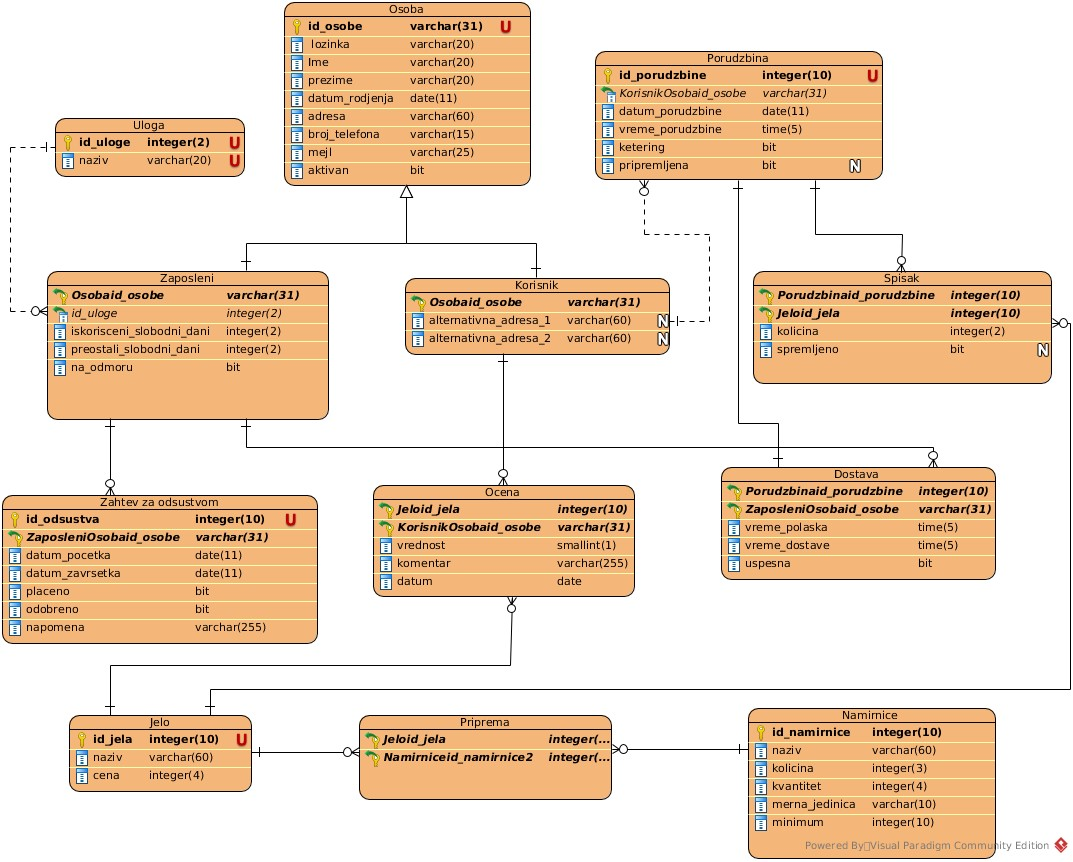
\includegraphics[width=1.1\textwidth]{slike/Baza.jpg}
    \end{center}
    \caption{Dijagram baze podataka}
    \label{fig:slika_baza}
\end{figure}
\leavevmode

\newpage
\section{Arhitektura sistema}
\subsection{Osnovni prikaz}
Sledi prikaz karakteristika arhitekture informacionog sistema za poručivanje hrane jednog restorana. Odluke su donošene u skladu sa prirodom i funkcionalnim zahtevima sistema, kao i potrebama korisnika i razvijaoca.Time su određene sledeće karakteristike arhitekture informacionog sistema:
\begin{enumerate}
    \item Tip aplikacije: Veb aplikacija
    \item Strategije isporučivanje: jedan serverski i više klijentskih računara
    \item Odgovarajuće tehnologije: Java, JavaFX, MYSQL, JS, CSS
    \item Prateće komponente:
    \begin{enumerate}
        \item \textbf{Logovanje na sistem:} Podsistem za autentikaciju korisnika. Sadrži GUI komponentu za učitavanje klijentskih podataka i komponentu za validaciju podataka.
        \item \textbf{Backup baze:} Predstavlja podsistem za pravljenje kopija baze. Uz to, vodi računa o konzistentnosti kopija, intervalu backup-ovanja i sl.
        \item \textbf{Pomoć:} Sadrži uputstvo za upotrebu, kontakt i podršku.
        
    \end{enumerate}
\end{enumerate}

\subsection{Tip arhitekture i slojevi}
Arhitektura sistema je osmišljena kao klijent-server tip arhitekture čiji su entiteti bazirani na tri (odnosno četiri) sloja.
\begin{enumerate}
    \item \textbf{Model} sadrži skup klasa koje opisuju sve entitete iz informacionog sistema. Model se sastoji od sledećih klasa sa opisanom funkcijom:
    \begin{itemize}
        \item \emph{Korisnik} je klasa koja sadrži sve lične informacije o korisniku aplikacije. Njegova polja su identična kolonama u tabeli Osoba (slika 11), takođe sadrži i alternativne adrese koje jedan korisnik može imati.
        \item \emph{Zaposleni} je klasa koja sadrži sve lične informacije o zaposlenom u restoranu. Polja klase Zaposleni identična su kolonama u tabeli Osoba (slika 11), takođe sadrži i informacije o njegovoj ulozi o sistemu, broj broj preostalih/iskorišćenih slobodnih dana, kao i podatak da li je taj zaposleni trenutno na odmoru.
        \item \emph{ZahtevZaOdsustvom} je klasa koja sadrži sva polja istoimenog entiteta. U ovoj klasi, nalaze se sve potrebne informacije za obradu zahteva zaposlenog za odlazak na plaćeno/neplaćeno odsustvo kao što su datum\_početka i datum\_završetka, kao i informacija o tome da li je određeni zahtev prihvaćen ili odbijen.
        \item \emph{Namirnica} je klasa oja sadrži podatke o svakoj namirnici koja se trenutno nalazi u magacinu. Ona direktno oslikava entitet Namirnice koji se nalazi u bazi.
         \item \emph{Jelo} je klasa koja oslikava prikaz jednog jela u jelovniku koji se prikazuje korisniku.
         \item \emph {Priprema} je klasa koja sadrži id-jeve klase Jelo i klase Namirnice i predstavlja njihovu agregaciju. Pruža nam informaciju o tome koje namirnice ulaze u sastav jednog jela.
         \item \emph{Porudžbina} je klasa koja sadrži sve informacije koje se prosleđuju nakon što korisnik uputi zahtev za poručivanjem određenog jela. Sadrži informacije o korisniku koji prosleđuje zahtev tj. id korisnika i propratne opisne informacije za datu porudžbinu.
         \item \emph{Spisak} je klasa koja sadrži id objekta klase Porudžbina, kao i listu id-jeva objekata klase Jelo. Informacije iz ove klase nam pomažu da vidimo koja sve jela ulaze u sastav jedne određene porudžbine, koja je njihova količina, kao i to da li je određeno jelo trenutno spremljeno ili se na njega čeka.
         \item \emph{Dostava} je klasa koja sadrži id porudžbine sa kojom je data dostava povezana, id zaposlenog koji će da izvrši dostavu. Beleže se i informacije o tome da li je određena dostava uspešno obavljena i koliko je vremena trebalo dostavljaču da izvrši dostavu. 
    \end{itemize}
    \item \textbf{View} odnosno pogled prikazuje podatke iz modela, u formatu pogodnom za interakciju, kao komponentu korisničkog interfejsa. Za svaki slučaj upotrebe kreiran je jedan view. U zavisnosti od toga da li je osoba koja poseduje nalog zaposleni u restoranu ili korisnik koji poručuje hranu, prikazuju im se različiti interfejsi nakon logovanja na sistem. Ono što im je zajedničko je kartica \emph{Nalog} koju imaju i korisnik i zaposleni. Ovde se nalaze sve njihove lične informacije koje su uneli tokom registracije, od kojih određene mogu da ažuriraju, uklone ili dodaju.
    \item \textbf{Kontroler} sadrži pripremu podataka za pogled, proračune, kao i njihovu pripremu pre slanja na obradu modelu. On je u ovom slučaju izdeljen na dve komponente - klijent, odnosno server kontroler. Klijentska strana obavlja komunikaciju između pogleda i modela u zavisnosti od korisnikovog unosa, dok se na serverskoj instanci obavlja autentikacija, autorizacija, i upravljanje podacima.
\end{enumerate}

\begin{figure}[!ht]
    \leavevmode
    \centering
    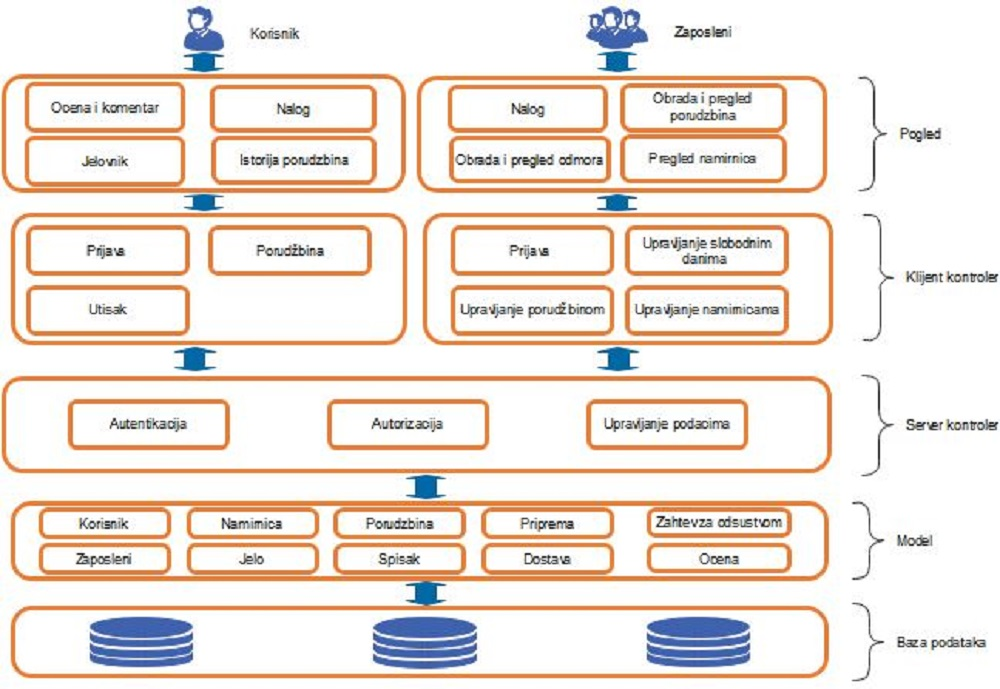
\includegraphics[width=1.2\textwidth]{slike/arhitektura.JPG}
    \caption{Arhitektura sistema}
    \label{fig:slika11}
\end{figure}
\leavevmode

% \input{}
% \input{}

\end{document}
